% Offizielle Beispieldatei für beamer-Vorlage aus tubslatex Version 0.3beta2
\documentclass[fleqn,11pt,aspectratio=43]{beamer}

\usepackage[ngerman]{babel}
\usepackage[utf8x]{inputenc}
\usepackage{graphicx}
\usetheme[%
  %nexus,%        Nexus Fonts benutzen
  %lnum,%         Versalziffern verwenden
  %cmyk,%<rgbprint>,          Auswahl des Farbmodells
  blue,%<orange/green/violet> Auswahl des Sekundärfarbklangs
  dark,%<light,medium>        Auswahl der Helligkeit
  %colorhead,%    Farbig hinterlegte Kopfleiste
  %colorfoot,%    Farbig hinterlegt Fußleiste auf Titelseite
  colorblocks,%   Blöcke Farbig hinterlegen
  %nopagenum,%    Keine Seitennumer in Fußzeile
  %nodate,%       Kein Datum in Fußleiste
  tocinheader,%   Inhaltsverzeichnis in Kopfleiste
  %tinytocinheader,% kleines Kopfleisten-Inhaltsverzeichnis
  %widetoc,%      breites Kopfleisten-Inhaltsverzeichnis
  %narrowtoc,%    schmales Kopfleisten-Inhaltsverzeichnis
  %nosubsectionsinheader,%  Keine subsections im Kopfleisten-Inhaltsverzeichnis
  %nologoinfoot,% Kein Logo im Fußbereich darstellen
  ]{tubs}

% Titelseite
\title{Dynamic parallelism using CUDA}
\subtitle{The shallow water equation on an adaptive grid}
\author{Marc Kassubeck, Torsten Thoben}
% Titelgrafik, automatisch beschnitten, Weitere Optionen: <scaled/cropx/cropy>
% \titlegraphic[cropped]{\includegraphics{infozentrum.jpg}}
\titlegraphic[scaled]{\includegraphics{titlepicture.jpg}}

% Logo, dass auf Titelseiten oben rechts und auf Inthaltsseiten unten rechts
% dargestellt wird. Es wird jeweils automatisch skliert
\logo{\includegraphics{logo_wire_kreis.jpg}}
%\logo{Institut für Unkreativität\\und Schreibschwäche}

\begin{document}

\begin{frame}[plain]
\titlepage
\end{frame}

\begin{frame}{Inhalt}
\tableofcontents
\end{frame}


\section{The task}
\begin{frame}{The Task}
	\begin{itemize}
		\item Extension of an existing shallow water sovler
		\item With dynamic prallelism (DP)
	\end{itemize}
	\centering
	\includegraphics[width=0.8\textwidth]{dynamicparallelism.png}
\end{frame}

\section{Dynamic parallelism using CUDA}

\subsection{Implementation of DP with CUDA}	
\begin{frame}[fragile]{Implementation of DP with CUDA}
	\begin{itemize}
		\item DP in CUDA means calling a kernel inside a kernel
		\item So every thread calls a new grid
	\end{itemize}

	\begin{verbatim}
		main(){
		    ...
		    func <<< g,b >>> (depth);
		}
	\end{verbatim}	

	\begin{verbatim}
		__global__ void func(int depth){
		    ...
		    if(depth<2)
		        func  <<< g, b >>> (depth+1);
		}
	\end{verbatim}
\end{frame}

\subsection{DP and Synchronisation}
\begin{frame}{DP and Syncronisation}
	\begin{itemize}
		\item Father-kernel finished if his subgrid is finished but can continue working after the subkernel call
		\item To synchronize between one thread and his subgrids use \texttt{cudaDeviceSynchronize()} ($\neq$ \texttt{\_\_syncthreads()})
	\end{itemize}
	\centering
	\includegraphics[width=0.8\textwidth]{nesting-of-grids.png}
\end{frame}


\subsection{Recursion Depth and Device Limits}
\begin{frame}[fragile]{Recursion Depth and Device Limits}
	\begin{itemize}
		\item Nesting depth (hardware-limit is 24)
			\begin{itemize}
				\item Need to reserve a buffer for running/suspended or launching kernels
				\item \texttt{cudaDeviceSetLimit( cudaLimitDevRuntimePendingLaunchCount, x)}
				\item Default is set to 2048
			\end{itemize}
		\item Synchronization depth
			\begin{itemize}
				\item \texttt{cudaDeviceLimit(cudaLimitDevRuntimeSyncDepth, x)}
				\item Default is set to 2
			\end{itemize}
	\end{itemize}
\end{frame}


\section{The Problem}
	\begin{frame}{Problem: Implementation of the datastructure}
		\begin{itemize}
			\item Datastructure: Forest (many Trees)
			\item Limit to coarseness is the \texttt{forestsize} (number of trees)
			\item Limit to getting fine end up to the maximum recursions
			\item Trees: eg Quadtrees, Octrees...
		\end{itemize}
		\centering	
		\includegraphics[width=0.8\textwidth]{dynamicparallelism.png}	
	\end{frame}
\subsection{First try}

\begin{frame}[fragile]{GPU Datastructure using pointer}
	\begin{verbatim}
			class LeafElem : public TreeElem
			{
			public:
  			float value;
  			__device__ __host__ LeafElem();
  			virtual __device__ __host__ ~LeafElem(){};
  			virtual __device__ __host__ bool isLeaf()
  			{
    			return true;
  			}
			};
	\end{verbatim}
\end{frame}

\begin{frame}[fragile]{GPU Datastructure using pointer}
	\begin{verbatim}
			class BranchElem : public TreeElem
			{
			 public:
			    int nx;
			    int ny;
			    int depth;
			    TreeElem** children;
			    __device__ __host__ BranchElem(int nx, int ny, int depth);
			    virtual __device__ __host__ ~BranchElem();
			    virtual __device__ __host__ bool isLeaf()
			    {
			        return false;
			    }
			 };
	\end{verbatim}
\end{frame}

\begin{frame}{But this fails}
	\begin{center}
	
\includegraphics[width=1\textwidth]{fehler.png}
	\end{center}
	\begin{itemize}
		\item Kernel calls take too long to execute (> 7 seconds)
		\item Possible causes:
		\begin{itemize}
			\item Exponentially growing trees 
			\item Overhead to launch subgrids
			\item No coalesced memory access with pointers of this data structure
		\end{itemize}
	\end{itemize}
\end{frame}

\subsection{Back to Arrays}
	\begin{frame}{Storing the tree-structure in an Integer array}
		\centering
		\begin{tabular}{ | c | c | c | c || c | c | c | c |}
			\hline
  			0 & 0 & 0 & 0 & 1 & 1 & 2 & 2 \\ \hline
  			0 & 0 & 0 & 0 & 1 & 1 & 2 & 2 \\ \hline
  			0 & 0 & 0 & 0 & 1 & 1 & 1 & 1 \\ \hline
			0 & 0 & 0 & 0 & 1 & 1 & 1 & 1 \\ \hline \hline
  			0 & 0 & 0 & 0 & 0 & 0 & 0 & 0 \\ \hline
  			0 & 0 & 0 & 0 & 0 & 0 & 0 & 0 \\ \hline
  			0 & 0 & 0 & 0 & 0 & 0 & 0 & 0 \\ \hline
  			0 & 0 & 0 & 0 & 0 & 0 & 0 & 0 \\ \hline
		\end{tabular}
		\begin{itemize}
			\item Integer values denote the level in the tree
			\item The higher the value, the finer the grid will be in this area
			\item Solution values are averaged and stored in all corresponding 'supercells'
			\item Allows for better coalesced memory access
		\end{itemize}
	\end{frame}
	
\subsection{Results and discussion}
	\begin{frame}{Profiling}
		\centering
		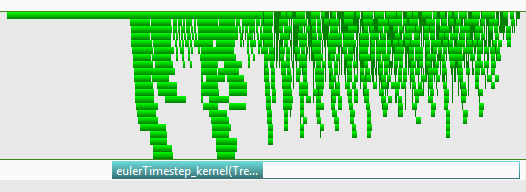
\includegraphics[width=1\textwidth]{profilingArray.png}
	\end{frame}
	
	\begin{frame}{Results}
		\centering
		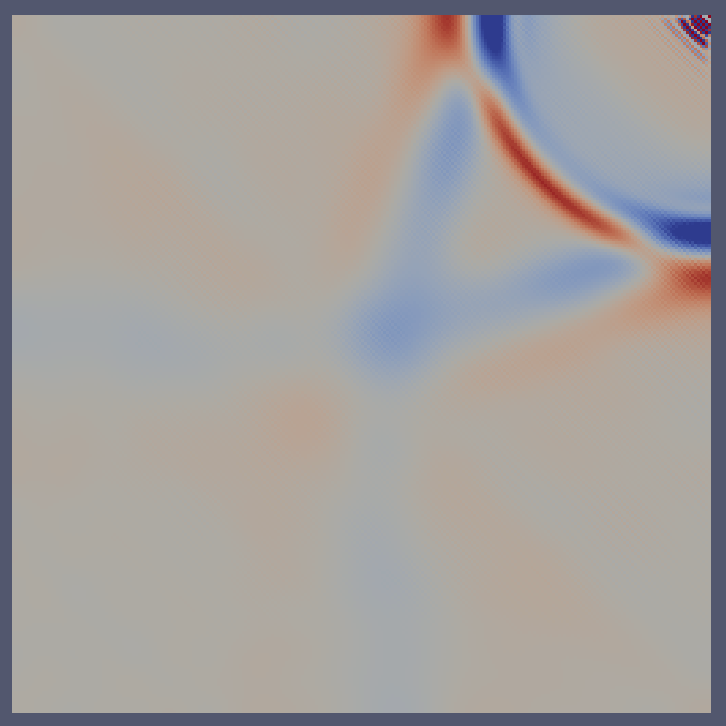
\includegraphics[height=\textheight]{res.png}
	\end{frame}
	
	\begin{frame}{Problems}
		\begin{itemize}
			\item Unfortunately this is still the solution using the original solver
			\item Some problems surfaced, when implementing the dynamic version
			\item Implementing the memory using CUDA Unified memory:
			\begin{itemize}
				\item On the one hand no \texttt{cudaMemcpy}
				\item On the other hand many calls to \texttt{cudaDeviceSynchronize}
				\item Too much data transfer CPU $\leftrightarrow$ GPU
				\item Too slow using our current implementation
			\end{itemize}
			\item Problems in the solver code
			\begin{itemize}
				\item Solutions may contain $\infty$ or \texttt{\#INDEFINITE}
				\item Maybe stability issue
				\item Maybe bug in solver code
			\end{itemize}
		\end{itemize}
	\end{frame}

\end{document}
